\documentclass[10pt,a4paper]{article}
%
%\sloppy
%
\setlength{\textwidth}{16cm}
\setlength{\textheight}{26.0cm}
\addtolength{\hoffset}{-1.6cm}
\addtolength{\voffset}{-4cm}

\usepackage[utf8]{inputenc}
\usepackage[spanish, es-tabla]{babel}
\usepackage{ae}
\usepackage{graphicx}

\usepackage{subcaption}
\usepackage{tikz,pgfplots}
%\pgfplotsset{compat=1.14}
\usepackage{epsfig}
\usepackage{setspace}

\usepackage{amsmath,amssymb,amsthm}
\usepackage{multicol, array}
\decimalpoint

\usepackage{sectsty}
\allsectionsfont{\mdseries \raggedright}
\sectionfont{\fontsize{14}{15}\selectfont}
\chapterfont{\large\sc\centering}
\chaptertitlefont{\centering}
\subsectionfont{\fontsize{12}{15}\selectfont}
\subsubsectionfont{\fontsize{12}{15}\selectfont}

\usepackage[T1]{fontenc}
\usepackage{textcomp}
\usepackage[slantedGreek]{mathpazo} %% ver psnfss2e
\usepackage{pifont}
\usepackage{newcent}
\usepackage[font = footnotesize, labelfont = bf, margin=20pt, tableposition=top]{caption}
\usepackage{xcolor}
\usepackage{listings}
\usepackage{fancyhdr}
\setlength{\headheight}{27pt}


\setlength{\parskip}{2mm}



\usepackage{xcolor}
\usepackage{listings}
\usepackage{lipsum}


\lstset{%
  language=R, literate =  {á}{{\'a}}1 {é}{{\'e}}1 {í}{{\'{\i}}}1 {ó}{{\'o}}1 {ú}{{\'u}}1 {Á}{{\'A}}1 {É}{{\'E}}1 {Í}{{\'I}}1 {Ó}{{\'O}}1 {Ú}{{\'U}}1 {ü}{{\"u}}1 {Ü}{{\"U}}1 {ñ}{{\~n}}1 {Ñ}{{\~N}}1,
  backgroundcolor=\color{gray!10!},
  classoffset=0,
  basicstyle=\ttfamily\tiny,
  showspaces=false,
  showstringspaces=false,
  keywordstyle=\color{blue!60!black},
  stringstyle=\color{blue},
  numbers=none,
  %numberstyle=\ttfamily\tiny,
  commentstyle=\color{verde}\textbf,
  morecomment=[l][\color{verde}\textbf]}




\usepackage{hyperref}
\hypersetup{
    colorlinks=true,
    linkcolor=blue,
    filecolor=black,      
    urlcolor=blue,
    citecolor=black,
    anchorcolor=black
}
 
\urlstyle{same}

\usepackage{fancyhdr}


\setlength{\parskip}{2mm}


\theoremstyle{definition}
\newtheorem{example}{Ejercicio N$^o$}

\begin{document}

\begin{center}
\begin{large}\bf{Parcialito - Laboratorio N$^o$ 4:} \end{large} \\
\end{center}

\begin{itemize}
\item[a)] Calcule la densidad de un esfera sólida de masa $m= (10.0 \pm 0.2) kg$ y radio $r= (0.650 \pm 0.001)dm$ ($1 dm = 10cm$). 
 
\item[b)] Si tiene 10 esferas del mismo material compacto, y conoce la masa y el radio de cada una... ¿Qué gráfica debe realizar para que a partir de un ajuste lineal pueda obtener la dimensión efectiva o topológica de las esferas? Anote las ecuaciones que tuvo en cuenta para contestar la pregunta anterior.

\item[c)] Teniendo en cuenta la siguiente tabla, haga las comparaciones de magnitudes correspondientes y estime de qué material está hecha la esfera del primer punto.
\end{itemize}

\begin{figure}[h!] 
\begin{center}
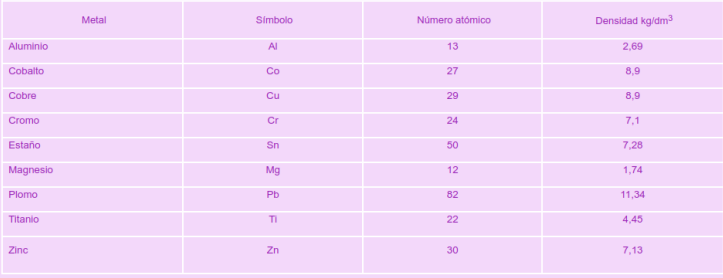
\includegraphics[width=140mm]{tabla.jpg}
\caption{Tabla de materiales con sus respectivas densidades, considere que el error es el 10$\%$ del valor central para cada valor de densidad.}
\end{center}
\end{figure}

\----------------------------------------------------------------------------------------------------------------------------------

\begin{center}
\begin{large}\bf{Parcialito - Laboratorio N$^o$ 4:} \end{large} \\
\end{center}

\begin{itemize}
\item[a)] Calcule la densidad de un esfera sólida de masa $m= (10.0 \pm 0.2) kg$ y radio $r= (0.650 \pm 0.001)dm$ ($1 dm = 10cm$). 
 
\item[b)] Si tiene 10 esferas del mismo material compacto, y conoce la masa y el radio de cada una... ¿Qué gráfica debe realizar para que a partir de un ajuste lineal pueda obtener la dimensión efectiva o topológica de las esferas? Anote las ecuaciones que tuvo en cuenta para contestar la pregunta anterior.

\item[c)] Teniendo en cuenta la siguiente tabla, haga las comparaciones de magnitudes correspondientes y estime de qué material está hecha la esfera del primer punto.

\begin{figure}[h!] 
\begin{center}
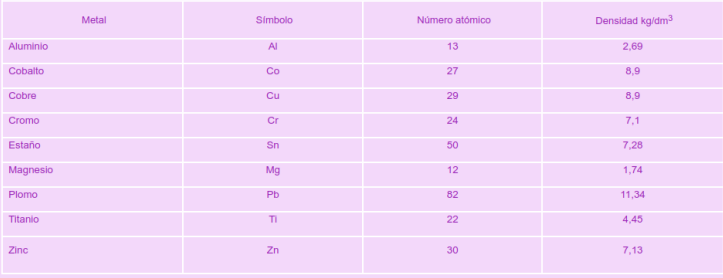
\includegraphics[width=140mm]{tabla.jpg}\nonumber  
\caption{Tabla de materiales con sus respectivas densidades, considere que el error es el 10$\%$ del valor central para cada valor de densidad.}
\end{center}
\end{figure}


\end{itemize}



 \end{document}
